\documentclass{article}
\usepackage{afterpage}
\usepackage{amsmath}
\usepackage{amssymb}
\usepackage{bbm}
\usepackage[legalpaper,margin=2cm,top=2cm,bottom=2cm]{geometry}
%\usepackage[legalpaper]{geometry}
\usepackage{graphicx}
\usepackage[utf8]{inputenc}
\usepackage[T1, T2A]{fontenc}
\usepackage[english,russian]{babel}
\usepackage{pdflscape}

\bibliographystyle{unsrt}

\DeclareMathOperator{\diag}{diag}
\DeclareMathOperator{\Arg}{Arg}

\newcommand{\bra}{\langle}
\newcommand{\ket}{\rangle} 

\graphicspath{ {images/} }

\begin{document}
    \begin{titlepage}
	\centering
	{\scshape\LARGE Московский физико--технический институт\par}
	{\scshape Кафедра проблем физики и астрофизики \par}
	\vspace{1cm}
	{\scshape\Large Отчёт о научной работе за 2 семестр 2016--2017 учебного года\par}
	\vspace{1.5cm}
	{\huge\bfseries Стабильность краевых состояний в топологических изоляторах
        \par}

	\vspace{2cm}
	{\Large\itshape Аникин Евгений\par}
	\vfill
	научный руководитель\par
	чл.-к.~РАН~д.~ф--м.~н.~П.И. \textsc{Арсеев}

	\vfill

% Bottom of the page
	{\large \today\par}
\end{titlepage}

    \tableofcontents
    	\newpage
%	\begin{abstract}
%        Из модели сильной связи для полупроводника с сильным спин--орбитальным
%        расщеплением выведен эффективный гамильтониан квантовой ямы.
%        Показано, что этот гамильтониан описывает топологический изолятор.
%        Для эфективного гамильтониана найден спектр одиночной примеси.
%	\end{abstract}
	\section{Введение}
    Двумерные топологические изоляторы --- это двумерные кристаллы 
    с особого рода зонной структурой:
    в них невозможно однозначно задать фазу функций 
    Блоха во всей зоне Бриллюэна. Причина этого в том, что (в простейшем случае) 
    отличен от нуля
    топологический инвариант \cite{Kohmoto1985}
    \begin{equation}
        \label{TKNN}
        N = \frac{1}{2\pi i} 
            \int d^2 k\, \left[\partial_i \langle u | \partial_j u \rangle -
            \partial_j \langle u | \partial_i u \rangle \right]
    \end{equation}
    В реалистичном случае этот инвариант отличен от нуля для каждой из компонент спина,
    но имеет для них противоположные знаки.
    Этот инвариант определяет спин--холловскую проводимость, 
    измеренную в квантах 
    магнитного потока:
    \begin{equation}
        \sigma_{xy} = \frac{e^2}{2\pi \hbar} N
    \end{equation}
    
    Наконец, точно так же, как в эффекте Холла, 
    на границе топологических изоляторов всегда возникают краевые состояния,
    пересекающие запрещённую зону, см. \cite{Hasan2010}.

    Эти краевые состояния обладают свойством киральности: электроны со спином 
    вверх движутся в одну сторону, а со спином вниз --- в другую. Кроме того, состояния 
    с разным направлением движения составляют крамерсовский дублет. Поэтому
    эти состояния не могут рассеиваться друг в друга 
    под действием какого--либо возмущения, то есть граница топологического 
    изолятора представляет из себя идеальный одномерный проводник.

    В многочисленных экспериментах (например, \cite{Konig2007}, \cite{Gusev2011})
    показано, что квантовая яма HgTe является топологическим изолятором при 
    некоторых параметрах. Наличие краевых состояний подтверждается измерениями
    нелокального сопротивления. Однако, хотя краевые состояния и
    определяют транспорт в квантовой яме, этот транспорт оказывается не баллистическим 
    \cite{Gusev2011}.
    Поэтому представляют интерес механизмы, которые могут приводить
    к рассеянию краевых мод друг в друга, либо иные механизмы, приводящие к неидеальности
    краевого транспорта.

    Целью настоящей работы является исследование влияние глубоких примесей на краевой 
    транспорт. Имеются в виду такие примеси, для которых энергия связанного состояния
    лежит внутри щели. Это, казалось бы, открывает возможность переходов краевых
    состояний в примесные и наоборот, и может приводить к изменению проводимости.
    

%#    Целью настоящей работы является изучение нескольких механизмов, которые
%#    потенциально могут приводить к рассеянию краевых состояний. Мы рассмотрели 
%#    точечную примесь в топологическом изоляторе, нашли для неё связанные состояния 
%#    и обсудили возможность образования примесных уровней в запрещённой зоне. 
%#    (Похожие вещи обсуждались в \cite{Lu2011}. Также 
%#    методом прямой диагонализации показана устойчивость краевых состояний к сильным
%#    потенциальным примесям и, наоборот, локализация магнитным беспорядком. Наконец, 
%#    обсуждается возможность спонтанного нарушения симметрии около края, вследствие чего
%#    краевые состояния перестают быть защищёнными. Все вычисления проделаны в эффективной
%#    модели сильной связи, описывающей два уровня размерного квантования квантовой ямы
%#    HgTe. 
    
%    Топологические изоляторы реализованы экспериментально в квантовых ямах $HgTe$. 
%    Теллурид ртути --- узкозонный полпроводник, 
%    Только системы со спин--орбитальным 
%    взаимодействием могут быть топологическими изоляторами. Впервые 
%    Дело в том, что холловская проводимость неинвариантна по отношению к обращению
%    времени, поэтому в системе с $\mathrm{T}$--симметрией, каковой является кристалл 
%    при отсутствии магнитного поля, и при от отсутствии спин--орбитального взаимодействия
%    $N$ обязательно равно нулю. Иная ситуация возникает, когда есть
%    спин--орбитальное взаимодействие. В этом случае $N$ может быть отлично от нуля
%    для каждой из компонент спина. 

    


    

    \section{Топологический изолятор на основе квантовой ямы HgTe}
    

    \subsection{Модель сильной связи для топологического изолятора}
Можно написать эквивалентный гамильтониан сильной связи. Блок
для одной компоненты спина будет иметь следующий вид (для простоты предполагается симметрия
зон):
\begin{equation}
    \label{BHZ}
    H = \left(\begin{matrix}
            \xi + \frac{1}{m}(2 - \cos{p_x} - \cos{p_y}) & 2t(\sin{p_x} - i\sin{p_y})   \\
            2t(\sin{p_x} + i\sin{p_y}) & - \xi - \frac{1}{m}(2 - \cos{p_x} - \cos{p_y}) \\
        \end{matrix}\right)
\end{equation}
Спектр этого гамильтониана несложно вычислить:
\begin{equation}
    E_p^2 = (\xi + \frac{1}{m}(2 - \cos{p_x} - \cos{p_y}))^2 + 4t^2(\sin^2{p_x} + \sin^2{p_y})
\end{equation}
Как видно, гамильтониан описывает две симметричные зоны, щель между которыми равна $2|\xi|$. 
При малых $k$ $E_p^2 = \xi^2 + (4t^2 + \xi/m)k^2$, то есть спектр дираковский.

В координатном (решёточном) представлении гамильтониан выглядит так:
\begin{multline}
    \label{BHZ_tight_binding}
    H_{\mathrm{lattice}} = \sum_{mn} \left\{
        a_{mn}^\dagger\left( \left(\xi + \frac{2}{m}\right) a_{mn}
                 -\frac{1}{2m}(a_{m+1,n} + a_{m-1,n} + a_{m,n+1} + a_{m,n-1})\right)\right. \\
        -it a_{mn}^\dagger(b_{m+1,n} -b_{m-1,n} - i(b_{m,n+1} - b_{m,n-1}))\\
        -it b_{mn}^\dagger(a_{m+1,n} -a_{m-1,n} + i(a_{m,n+1} - a_{m,n-1}))\\
        -\left. b_{mn}^\dagger\left( \left(\xi + \frac{2}{m}\right) b_{mn}
                 -\frac{1}{2m}(b_{m+1,n} + b_{m-1,n} + b_{m,n+1} + b_{m,n-1})\right) \right\}
\end{multline}
Здесь $a_{mn}$, $b_{mn}$ --- операторы уничтожения состояний двух зон 
соответственно на узле $(m,n)$. Непосредственно обобщая этот решёточный гамильтониан, можно
рассматривать решётку конечного размера, добавлять примеси и так далее. 

    \section{Краевые состояния}
Рассмотрим одномерную цепочку \eqref{ham1d} с возмущением \eqref{pert} и устремим $\Delta E$
к бесконечности. Физически это означает добавление бесконечно высокой потенциальной стенки,
в результате чего мы получаем две полуцепочки, не связанные между собой. Далее можно 
обычным способом искать локализованные состояния. (Они называются таммовскими, так 
как впервые были рассмотрены Таммом, см. \cite{Tamm1933}, \cite{Shockley1939})

Разумеется, сказанное относится не только к цепочке \eqref{ham1d}, но и к любой другой модели
сильной связи. Всегда можно ввести такое возмущение, которое разделит систему на две
несвязанные части. Например, в случае плоскости возмущение должно быть примерно таким:
\begin{equation}
	\hat{V} = \Delta E \sum_m a^\dagger_{m,0} a_{m,0}, \quad \Delta E \to \infty
\end{equation}
Это означает, что мы добавляем целую линию примесных атомов с очень большой энергией.

В частном случае гамильтониана \eqref{ham1d} функция Грина получается такой:
\begin{multline}
	G^R(\omega, m,n) = G^R_0(\omega, m,n) - 
		\frac{G^R_0(\omega, m,0)G^R_0(\omega, 0, n)}{G^R_0(\omega,0,0)} = \\
		= \frac{e^{-|m-n|\kappa} - e^{-|m|\kappa- |n|\kappa}}{2t\sinh \kappa}
\end{multline}
Здесь нет локализованных состояний: у функции Грина нет изолированных полюсов. Локализованные
состояния возникают в более сложных случаях, некоторые из которых будут рассмотрены ниже.

\section{Два примера одномерной цепочки}
Так как в самой простой цепочке локализованных состояний не оказалось, усложним цепочку.
А именно, рассмотрим цепочку чередующихся атомов с разными свойствами. 

Во--первых, можно рассмотреть цепочку, где все матричные элемементы перехода между 
соседними атомами одинаковы, а энергии атомов различаются. Гамильтониан такой цепочки ---
\begin{equation}
	H = \sum_n \xi(a_n^\dagger a_n - b_n^\dagger b_n) + ta_n^\dagger(b_n + b_{n-1}) +
			ta_n(b_n^\dagger + b_{n-1}^\dagger)
\end{equation}
Во--вторых, возможен случай, когда энергии атомов одинаковы, но, напротив, различаются 
матричные элементы. Гамильтониан в этом случае ---
\begin{equation}
	H = \sum_n t_1(a_n^\dagger b_n + a_n b_n^\dagger) + 
		t_2 (a_{n+1}^\dagger b_n + a_{n+1} b_n^\dagger)
\end{equation}
Оказывается, что краевое состояние есть только у второй цепочки, причём его наличие 
зависит от типа последней связи в решётке.

Рассмотрим подробнее вторую цепочку. Без ограничения общности будем считать, что
$t_1 > t_2 > 0$ .

После преобразования Фурье гамильтониан примет вид
\begin{equation}
	H = \sum_p 
			(t_1 e^{-\frac{ipa}{2}} + t_2 e^{\frac{ipa}{2}}) a_p^\dagger b_p + 
			(t_1 e^{\frac{ipa}{2}} + t_2 e^{-\frac{ipa}{2}}) a_p b_p^\dagger
\end{equation}
Отсюда получаем энергетический спектр, содержащий две зоны.
\begin{equation}
	E_p^{1,2} = \pm \epsilon_p = \pm|t_1 e^{\frac{ipa}{2}} + t_2 e^{-\frac{ipa}{2}}| = 
		\pm\sqrt{t_1^2 + t_2^2 + 2t_1t_2 \cos{pa}}
\end{equation}
Введём обозначение 
Гамильтониан диагонализуется преобразованием
\begin{equation}
	\left(
	\begin{matrix}
		a_p \\
		b_p
	\end{matrix}
	\right)
	=
	\frac12
	\left(
	\begin{matrix}
		1 & -e^{i\phi}	\\
		e^{-i\phi} & 1
	\end{matrix}
	\right)
	\left(
	\begin{matrix}
		x_p \\
		y_p
	\end{matrix}
	\right),
\end{equation}
\begin{equation}
	e^{i\phi} = \frac{t_1 e^{-\frac{ipa}{2}} + t_2 e^{\frac{ipa}{2}}}
				{\sqrt{t_1^2 + t_2^2 + 2t_1t_2 \cos{pa}}}
\end{equation}
Отсюда получаются выражения для функций Грина в импульсном представлении:
\begin{equation}
	\label{gaa}
	G^R_0 (\omega, p, A, A) =  G^R_0 (\omega, p, B, B) = \frac{1}{2}\left(
		\frac{1}{\omega - \epsilon_p + i\delta} + 
					\frac{1}{\omega + \epsilon_p + i\delta}\right)
\end{equation}
\begin{equation}
	G^R_0 (\omega, p, A, B) = \frac12 \left(\frac{e^{i\phi}}{\omega - \epsilon_p + i\delta} -
						\frac{e^{i\phi}}{\omega + \epsilon_p + i\delta} \right)
\end{equation}
\begin{equation}
	G^R_0 (\omega, p, B, A) = \frac12 \left(\frac{e^{-i\phi}}{\omega - \epsilon_p + i\delta} -
						\frac{e^{-i\phi}}{\omega + \epsilon_p + i\delta} \right)
\end{equation}
Здесь аргументы $A$, $B$ соответствуют операторам $a_p$ и $b_p$. 

Чтобы рассмотреть половину цепочки, введём возмущение 
$V = \Delta E a_0^\dagger a_0$, где $\Delta E$ очень велико.
Это приведёт к уже знакомому нам уравнению Дайсона. Его решение --- 
\begin{multline}
	G^R(\omega, m, s, n, s') = 
		G^R_0(\omega, m,s,n,s') - 
		\frac{G^R_0(\omega, m, s, 0, A)G^R_0(\omega, 0, A, n, s')}{G^R_0(\omega, 0, A, 0, A)},\\
		s,s' = A,B
\end{multline}
Уровни энергии даются, как видно, нулями функции $G^R_0(\omega, 0,A,0,A)$, а волновая функция
связанного состояния пропорциональна $G^R_0(\omega, m,s,0,A)$.

В нашем случае, как нетрудно убедиться, этот уровень энергии --- $E = 0$. Действительно, подставим 
$\omega = 0$ в (\ref{gaa}). Получается
\begin{equation}
	G^R_0 (\omega, p, A, A) = 
		-\frac{1}{2\epsilon_p} + 
					\frac{1}{2\epsilon_p} = 0
\end{equation}
Отсюда следует, что функции Грина в узельном представлении, 
составленные из операторов $a$, обращаются в нуль для всех $m,n$, и, таким образом, волновая 
функция связанного состояния равна нулю во всех узлах $a$. 

Волновая функция оказывается равной 
\begin{equation}
	\begin{split}
	\psi(n,A) &  = 0, \\
	\psi(n, B) & = 
	\left\{
	\begin{matrix}
		{\displaystyle
 		\sqrt{1 - \left(\frac{t_2}{t_1}\right)^2}(-1)^n \left(\frac{t_2}{t_1}\right)^n}
									&	\quad \mbox{при} \quad n \ge 0 \\
		0 & \quad \mbox{при} \quad n < 0
	\end{matrix}
	\right.,\\
	\end{split}
\end{equation}

Краевое состояние есть только у правой половины цепочки, у которой последнее перекрытие --- 
$t_2$, то есть маленькое.

Теперь рассмотрим цепочку с одинаковыми элементами перекрытия. Все вычисления для неё
проводятся точно так же, поэтому просто приведём их результаты:
\begin{equation}
	E_p^{1,2} = \pm \epsilon_p = \pm \sqrt{\xi^2 + 4t^2 \cos^2{\frac{pa}{2}}}
\end{equation}
\begin{equation}
	\begin{split}
	G_0^R(\omega, p, A, A) = \frac{\omega + \xi}{\omega^2 - \epsilon_p^2 + i\delta}\\
	G_0^R(\omega, p, A, B) = \frac{2t\cos{pa}}{\omega^2 - \epsilon_p^2 + i\delta}\\
	G_0^R(\omega, p, B, B) = \frac{\omega - \xi}{\omega^2 - \epsilon_p^2 + i\delta}\\
	\end{split}
\end{equation}
Уровни энергии для системы с возмущением 
определяются уравнением $G_0^R(\omega,0,A,0,A) = 0$, или 
{\sloppy

}

\begin{equation}
	0=\int_{-\pi}^{\pi} \frac{dk}{2\pi} 
		\frac{\omega + \xi}{\omega^2 - \xi^2 - 2t^2 - 2t^2\cos{pa} + i\delta} 
\end{equation}
Интеграл обращается в ноль при $\omega = -\xi$, на границе непрерывного спектра. Внутри
запрещённой зоны, то есть в области $|\omega| < \xi$, интеграл строго отрицателен. Отсюда
можно заключить, что в этом случае граничного состояния не существует: никаких новых
полюсов у функции Грина не возникло.

    \section{Точечная примесь}
Гамильтониан простейшего топологического изолятора может быть записан в виде
\begin{equation}
    \label{BHZ}
    H = \left(\begin{matrix}
            \xi + \frac{1}{m}(2 - \cos{p_x} - \cos{p_y}) & 2t(\sin{p_x} - i\sin{p_y})   \\
            2t(\sin{p_x} + i\sin{p_y}) & - \xi - \frac{1}{m}(2 - \cos{p_x} - \cos{p_y}) \\
        \end{matrix}\right)
\end{equation}
Уровни энергии ---
\begin{equation}
    E_p^2 = (\xi + \frac{1}{m}(2 - \cos{p_x} - \cos{p_y}))^2 + 4t^2(\sin^2{p_x} + \sin^2{p_y})
\end{equation}
Если перейти из импульсного представления в координатное, то он превратится в гамильтониан
сильной связи. Гамильтониан примеси тогда можно записать в виде
\begin{equation}
    V = \Delta E (a_{00}^\dagger a_{00} + b_{00}^\dagger b_{00})
\end{equation}
\subsection{Энергия связанных состояний}
Связанные состояния даются уравнением
\begin{equation}    
    \det{\left[\mathbbm{1} - \Delta E \int \frac{d^2 p}{(2\pi)^2} 
            \frac{\omega + \hat{H}}{\omega^2 - E_p^2}\right]} = 1
\end{equation}
В последнем интеграле (от матрицы) недиагональные члены из--за симметрии обращаются в ноль.
Таким образом, связанные состояния сводятся к уравнениям
\begin{equation}
    \label{integrals}
    \left[
    \begin{split}
        &\int \frac{d^2 p}{(2\pi)^2} 
            \frac{\omega + \xi + \frac{1}{m}(2 - \cos{p_x} - \cos{p_y})}
                 {\omega^2 - E_p^2} = \frac{1}{\Delta E},\\
        &\int \frac{d^2 p}{(2\pi)^2} 
            \frac{-\omega + \xi + \frac{1}{m}(2 - \cos{p_x} - \cos{p_y})}
                 {\omega^2 - E_p^2} = -\frac{1}{\Delta E},
    \end{split}
    \right.
\end{equation}
Эти интегралы можно взять приближённо в круге небольшого радиуса $p_{\mathrm{max}}$,
если учесть, что при малых $p$ спектр близок к 
коническому. После интегрирования получается
\begin{equation}
    G(\omega,0,0)_{11} = -\frac{1}{8\pi}\frac{1}{m(4t^2 + \frac{\xi}{m})}
        \left[ p_{\mathrm{max}}^2 + 
            \left(2m(\omega+\xi) - \frac{\xi^2 - \omega^2}{4t^2 + \frac{\xi}{m}}\right) 
                \log{\left(1 + \frac{\left(4t^2 + \frac{\xi}{m}\right)p_{\mathrm{max}}^2}
                                    {\xi^2 - \omega^2}\right)}\right]
\end{equation}
Конечно, интегралы из \eqref{integrals} можно взять численно. Для 
$\xi, m, t = -0.03, 0.1, 0.5$ компоненты функции Грина изображены на графике.

\begin{figure}[h]
    \centering
    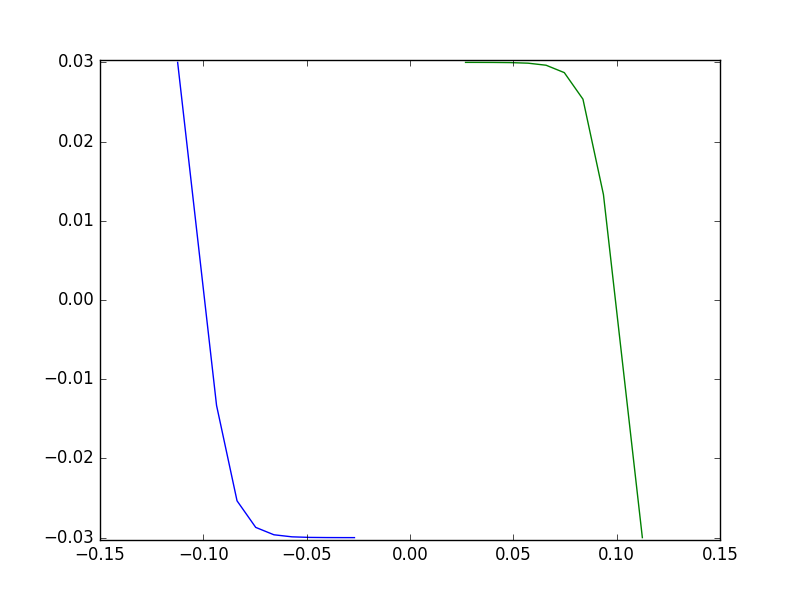
\includegraphics[width=0.8\linewidth]{impurity_levels.png}
    \caption{
            На графике показаны уровни энергии связанных состояний на точечной примеси. 
            По оси абсцисс отложена обратная глубина ямы, $\Delta E^{-1}$. <<Хвосты>>
            обоих графиков должны быть продолжены до бесконечности, у синего графика ---
            вправо снизу, у зелёного --- влево сверху. Видно,
            что при бесконечной глубине ямы имеются два слабо связанных состояния.
            }
\end{figure}

Вычисление выше показывает, что происходит на краях этого графика. А именно, ``хвосты'' 
функций Грина растут логарифмически до бесконечности.
Таким образом, для малых $\Delta E < 0$ появляется одно связанное состояние около 
зоны проводимости. При дальнейшем росте возмущения появляется состояние около валентной зоны.

\subsection{Волновые функции}
Волновые функции даются компонентами свободной
функции Грина:
\begin{equation}
    \Psi_{\alpha, i}(x) = G_0(x)_{\alpha i}
\end{equation}
Здесь $\alpha$ --- ``спинорный'' индекс, а $i$ --- индекс, соответствующий номеру волновой 
функции.

Функция Грина --- 
\begin{equation}
    G_0(x) = \int \frac{d^2 p}{(2\pi)^2} 
            \frac{\omega + \hat{H}}{\omega^2 - E_p^2} e^{ipx}
\end{equation}
Их можно вычислить с помощью формального трюка. Определим новую функцию
$F(x,y)$:
\begin{equation}
    F(x,y) = \equiv \int \frac{d^2 p}{(2\pi)^2} 
            \frac{e^{ip_x x + ip_y y}}{\omega^2 - E_p^2} 
\end{equation}
Несложно понять, что компоненты функций Грина выражаются (точными соотношениями)
 через $F(x,y)$. А именно,
\begin{equation}
    \label{differences}
    \begin{split}
        G_{11} & = (\omega + \xi) F(x,y) - 
            \frac{1}{m}(F(x+1,y) + F(x-1,y) + F(x,y+1) + F(x, y-1) - 4F(x,y))\\
        G_{21} & = -it(F(x+1,y) - F(x-1,y)) + t(F(x,y+1) - F(x,y-1))
    \end{split}
\end{equation}
С другой стороны, $F(x,y)$ может быть вычислена приближённо. Если разложить 
выражение в знаменателе около $p = 0$ и распространить интегрирование до $\infty$, то получится
сходящийся и берущийся интеграл.
\begin{equation}
    F(x,y) \approx -\int \frac{p\,dp\,d\cos{\theta}}{(2\pi)^2} 
        \frac{e^{ipr\cos{\theta}}}{\xi^2 - \omega^2 - (4t^2 + \frac{\xi}{m})p^2} = 
        -\frac{1}{2\pi} \frac{1}{4t^2 + \frac{\xi}{m}}
        K_0 \left(\sqrt{\frac{\xi^2 - \omega^2}{4t^2 + \frac{\xi}{m}}}R \right)
\end{equation}
Разности \eqref{differences} можно аппроксимировать производными. Пользуясь тем, что
$K_0(x)$ --- решение модифицированного уравнения Бесселя, получим 
\begin{equation}
    \begin{split}
        G_{11} & = -\frac{1}{2\pi} \frac{1}{4t^2 + \frac{\xi}{m}}
        \left( \omega + \xi - \frac{1}{m} \frac{\xi^2 - \omega^2}{4t^2 + \frac{\xi}{m}} \right)
        K_0 \left(\sqrt{\frac{\xi^2 - \omega^2}{4t^2 + \frac{\xi}{m}}}R \right)\\
        G_{21} & = \frac{it}{\pi} \sqrt{\frac{\xi^2 - \omega^2}
                                     {(4t^2 + \frac{\xi}{m})^{3}}}
        K_0' \left(\sqrt{\frac{\xi^2 - \omega^2}{4t^2 + \frac{\xi}{m}}}R \right)e^{i\theta}
    \end{split}
\end{equation}
%Найдём момент импульса найденных состояний. Оператор полного момента имеет вид
%\begin{equation}
%    J_z = x p_y - y p_x + \frac{1}{2}\sigma_z
%\end{equation}
%Несложно понять, что у двух найденных состояний полный момент равен $\pm \frac{1}{2}$.
%
%Интересно также найти магнитный момент. Оператор магнитного момента ---
%\begin{equation}
%    m_z = \frac{e}{2c}(x v_y - y v_x) + \frac{e}{2m_0c} \sigma_z
%\end{equation}
%Операторы скорости в низшем порядке по импульсам ---
%\begin{equation}
%    \begin{split}
%        v_x & = \begin{pmatrix} 
%                -\frac{i}{m} \partial_ x & 2t \\
%                2t & \frac{i}{m}\partial_x
%              \end{pmatrix} \\
%        v_y & = \begin{pmatrix} 
%                -\frac{i}{m} \partial_y & -2it \\
%                2it & \frac{i}{m}\partial_y
%              \end{pmatrix} \\
%    \end{split}
%\end{equation}
%Таким образом,
%\begin{equation}
%    m_z = \frac{e}{2mc}
%            \begin{pmatrix}
%               l_z & -2imt\cdot re^{-i\theta} \\
%               2imt\cdot r e^{i\theta} & -l_z
%            \end{pmatrix} + 
%          \frac{e}{2m_0c} \sigma_z
%\end{equation}

    \section{Численная диагонализация решёточного\\ гамильтониана}
Как уже говорилось, краевые состояния не рассеиваются на потенциальном беспорядке, 
если нет объёмных или примесных состояний с той же энергией. 
Это можно увидеть непосредственно, 
диагонализуя решёточный гамильтониан. Из результатов численной диагонализации видно, что
краевые состояния огибают глубокое препятствие (см. рис.~\ref{fig:obstacle}).
\begin{figure}[h]
    \centering
    \begin{minipage}[t]{0.4\linewidth}
        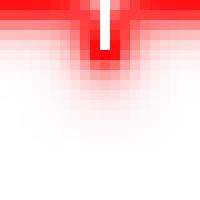
\includegraphics[width=0.9\linewidth]{obstacle_1.png}
    \end{minipage}
    \hfill
    \begin{minipage}[t]{0.4\linewidth}
        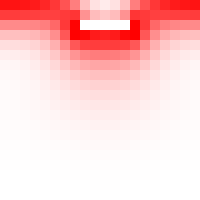
\includegraphics[width=0.9\linewidth]{obstacle_2.png}
    \end{minipage}
    \caption{
        Квадрат амплитуды волновой функции краевого состояния, огибающего препятствия. 
        Размер решётки --- $20\times20$, по горизонтальной оси наложены периодические
        граничные условия.
    }
    \label{fig:obstacle}
\end{figure}

Также краевые состояния <<выживают>> под действием даже довольно сильного потенциального
беспорядка
\begin{equation}
    \hat{V} = \sum_{m,n} V_{mn} (a_{mn}^\dagger a_{mn} + b_{mn}^\dagger b_{mn}),
\end{equation}
где $V_{mn}$ равномерно распределены по отрезку $[-\frac{W}{2}, \frac{W}{2}]$, см.
рис.~\ref{fig:disordered_stripe}.

\begin{figure}[h]
    \centering
    \begin{minipage}[h]{0.4\linewidth}
        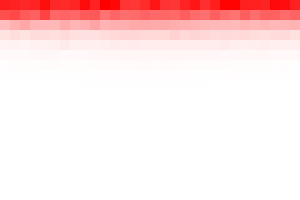
\includegraphics[width=1.\linewidth]{dis_edge_state_1.png}
        \caption{
            Волновая функция краевого состояния с беспорядком.
            Параметры модели: $\xi, m, t = -0.2, 1, 0.4$, сила беспорядка --- $0.5$.
            }
    \end{minipage}
    \hfill
    \begin{minipage}[h]{0.4\linewidth}
        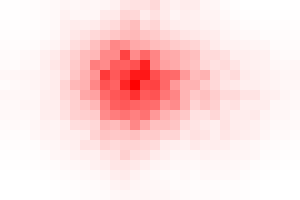
\includegraphics[width=1.\linewidth]{dis_bulk_state.png}
        \caption{
            Волновая функция объемного состояния с беспорядком для тех же параметров.
            }
    \end{minipage}
    \label{fig:disordered_stripe}
\end{figure}

Магнитный беспорядок, как нарушающий $T$--симметрию, приводит к рассеянию состояний
с двумя компонентами спина друг в друга. Это приводит к локализации краевых состояний,
что продемонстрировано на рис.~\ref{fig:magnetic_disorder}.  Магнитный беспорядок 
в симуляции имел вид
\begin{equation}
    \hat{V}_{\mathrm{mgn}} = \sum_{mn} J \hat{\sigma}_{mn} S_{mn},
\end{equation}
$\hat{\sigma}$ --- оператор спина на узле, $S_{mn}$ --- случайный вектор на единичной сфере.
\begin{figure}[h]
    \centering
    \begin{minipage}[h]{0.9\linewidth}
        \centering
        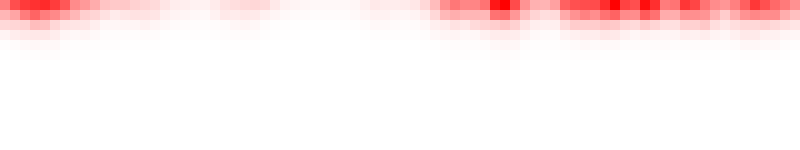
\includegraphics[width=0.7\linewidth]{mgn_edge_st_1.png}
    \end{minipage}
    \vfill
    \begin{minipage}[h]{0.9\linewidth}
        \centering
        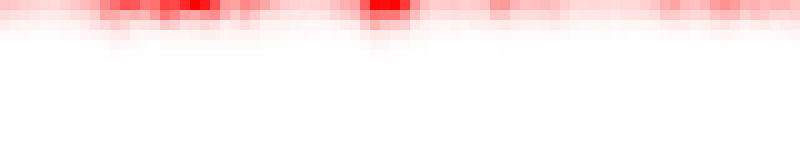
\includegraphics[width=0.7\linewidth]{mgn_edge_st_2.png}
    \end{minipage}
    \vfill
    \begin{minipage}[h]{0.9\linewidth}
        \centering
        
\includegraphics[width=0.7\linewidth]{mgn_edge_st_3.png}
    \end{minipage}
    \caption{
        Волновые функции краевых состояний с магнитным беспорядком 
        для тех же параметров.
        }
    \label{fig:magnetic_disorder}
\end{figure}

Также мы диагонализовали гамильтониан для случая, когда энергии примесных состояний
лежат в середине щели (см. рис.~\ref{fig:impurity_numeric_levels}). Для этого нужно
специальным образом подобрать силу возмущения.

\begin{figure}[h]
    \centering
    \begin{minipage}[h]{0.9\linewidth}
        \centering
        
\includegraphics[width=0.7\linewidth]{fig2.png}
    \end{minipage}
    \vfill
    \begin{minipage}[h]{0.9\linewidth}
        \centering
        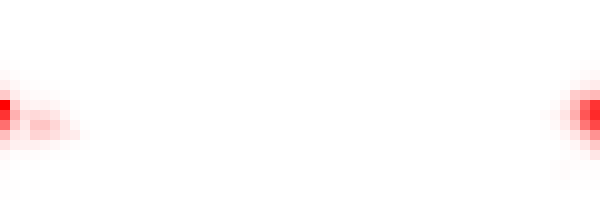
\includegraphics[width=0.7\linewidth]{fig3.png}
    \end{minipage}
    \vfill
    \begin{minipage}[h]{0.9\linewidth}
        \centering
        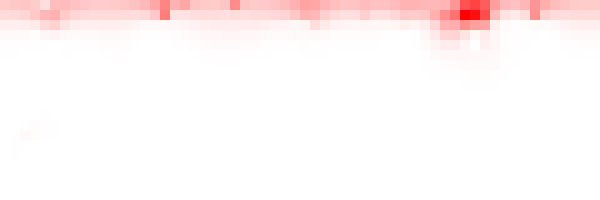
\includegraphics[width=0.7\linewidth]{fig5.png}
    \end{minipage}
    \caption{
        Волновые функции краевых состояний c примесями внутри щели      
    }

    \label{fig:magnetic_disorder}
\end{figure}

    \section{Спин--орбитальное взаимодейтвие в приближении сильной связи}
Необходимым ``ингредиентом'' для топологических изоляторов является спин--орбитальное 
взаимодействие. Экспериментальная реализация \cite{Bernevig2006, Konig2007} двумерного топологического изолятора ---
квантовая яма CdTe--HgTe--CdTe, составляющие которой --- узкозонные полупроводники с 
сильным спин--орбитальным расщеплением. Для их описания давно применяются
гамильтонианы Латтинжера и Кейна (\cite{Luttinger1956,Kane1957}). Однако эти гамильтонианы
выводятся из симметрийных соображений в $k\cdot p$ методе и, следовательно,
дают спектр только в центре зоны Бриллюэна, а также не слишком интуитивно понятны.

Мы построили простую модель сильной связи, аналогичную модели Кейна, 
учитывающую валентную $p$--зону и $s$--зону проводимости. Как показано, она переходит
в модель Кейна при малых $k$. Также она даёт возможность найти спектр во всей зоне 
Бриллюэна, а также интуитивно понятным образом описать одиночные примеси, границы образца,
резкие изменения параметров и прочее.

Модель представляет из себя 
кубическую решётку из атомов, на каждом из которых ``сидят'' состояния
с $p_x$--, $p_y$--, $p_z$-- и $s$--орбиталями и двумя 
возможными проекцими спина. В модели учитывались перекрытия
орбиталей соседних атомов, а также внутриатомное спин--орбитальное взаимодействие.
В литературе утверждается, что эффекты от межатомного спин--орбитального 
взаимодействия пренебрежимо малы.

Для написания
спин--орбитального гамильтониана $p$--зоны необходимо перейти к состояниям с определённым
полным моментом. Эти состояния выражаются через $p_x$, $p_y$, $p_z$ орбитали следующим образом:
\begin{equation}
	\label{transform1}
	\begin{gathered}
        \Psi_{\frac{3}{2},\frac{3}{2}} = \frac{X + iY}{\sqrt{2}}\alpha\\
        \Psi_{\frac{3}{2}, \frac{1}{2}} = \sqrt{\frac{1}{3}}\frac{X + iY}{\sqrt{2}}\beta -
                                         \sqrt{\frac{2}{3}} Z\alpha\\
        \Psi_{\frac{3}{2}, -\frac{1}{2}} = -\sqrt{\frac{1}{3}}\frac{X - iY}{\sqrt{2}}\alpha -
                                         \sqrt{\frac{2}{3}} Z\beta\\
        \Psi_{\frac{3}{2},-\frac{3}{2}} = -\frac{X - iY}{\sqrt{2}}\beta
	\end{gathered}
\end{equation}
\begin{equation}
	\label{transform2}
	\begin{gathered}
        \Psi_{\frac{1}{2}, \frac{1}{2}} = \sqrt{\frac{2}{3}}\frac{X + iY}{\sqrt{2}}\beta +
                                         \sqrt{\frac{1}{3}} Z\alpha\\
        \Psi_{\frac{1}{2}, -\frac{1}{2}} = -\sqrt{\frac{2}{3}}\frac{X - iY}{\sqrt{2}}\alpha-
                                         \sqrt{\frac{1}{3}} Z\beta\\
	\end{gathered}
\end{equation}
Здесь $X,Y,Z$ --- атомные орбитали, $\alpha,\beta$ --- состояния со спином вверх и вниз.

Как хорошо известно, в атоме гамильтониан спин--орбитального взаимодейстия имеет вид
\begin{equation}
    H_{\mathrm{SO}} =  A(\vec{S}, \vec{L}) = \frac{A}{2}(J^2 - L^2 - S^2)
\end{equation}
Если орбитальный момент фиксирован, то энергия определяется полным моментом. Таким образом,
спин--орбитальное взаимодействие приводит к расщеплению состояний с моментами $\frac32$ и
$\frac12$.

Пусть матричные элементы перекрытия $p$-- орбиталей --- $t_\parallel$ и $t_\perp$. Тогда
несложно показать, что гамильтониан тяжёлых и лёгких дырок в импульсном представлении ---
\begin{equation}
    \begin{gathered}
    H_v = \begin{bmatrix}
            H_l & H_r
        \end{bmatrix},\\
    H_l = 
    \begin{pmatrix}
        (t_\parallel + t_\perp)(\cos{p_x} + \cos{p_y}) + 2t_\perp \cos{p_z} & 0 \\
        0 & \left(\frac{t_\parallel}{3} + \frac{5t_\perp}{3}\right)(\cos{p_x}+\cos{p_y})+ 
                           \left(\frac{2t_\perp}{3} + \frac{4t_\parallel}{3}\right)\cos{p_z} \\
        -\frac{1}{\sqrt{3}}(t_\parallel - t_\perp)(\cos{p_x} - \cos_{p_y}) & 0 \\
        0 & -\frac{1}{\sqrt{3}}(t_\parallel - t_\perp)(\cos{p_x} - \cos_{p_y}) 
    \end{pmatrix}\\
    H_r = 
    \begin{pmatrix}
        -\frac{1}{\sqrt{3}}(t_\parallel - t_\perp)(\cos{p_x} - \cos_{p_y}) & 0 \\
        0 & -\frac{1}{\sqrt{3}}(t_\parallel - t_\perp)(\cos{p_x} - \cos_{p_y})\\
       \left(\frac{t_\parallel}{3} + \frac{5t_\perp}{3}\right)(\cos{p_x} + \cos{p_y}) + 
                    \left(\frac{2t_\perp}{3} + \frac{4t_\parallel}{3}\right)\cos{p_z} & 0 \\
        0 & (t_\parallel + t_\perp)(\cos{p_x} + \cos{p_y}) + 2t_\perp \cos{p_z}
    \end{pmatrix}
    \end{gathered}
\end{equation}
Э разумеется,ту матрицу можно разложить около нуля. Тогда получится хорошо известный 
гамильтониан Латтинжера \cite{Luttinger1956}:
\begin{equation}
    H_v = -\left(\gamma_1 + \frac{5}{2}\gamma_2\right) k^2 + 
        2\gamma_2(k_x^2J_x^2 + k_y^2J_y^2 + k_z^2J_z^2),
\end{equation}
где $J_i$ --- операторы момента для спина $\frac{3}{2}$, $\gamma_1 = \frac13 t_\parallel$,
$\gamma_2 = \frac16(t_\parallel - t_\perp)$, $\gamma_3 = 0$ (последнее слагаемое 
из гамильтониана Латтинжера опущено).

Теперь учтём перекрытие с $s$--зоной. Оно задаётся матрицей
\begin{equation}
    T = P\begin{pmatrix}
            -\frac{1}{\sqrt{2}}(\sin{p_x} + i\sin{p_y}) & \sqrt{\frac{2}{3}}\sin{p_z} &
             \frac{1}{\sqrt{6}}(\sin{p_x} - i\sin{p_y}) & 0 \\  
            0 & -\frac{1}{\sqrt{6}}(\sin{p_x} + i\sin{p_y}) & 
            \sqrt{\frac{2}{3}}\sin{p_z} & \frac{1}{\sqrt{2}}(\sin{p_x} - i\sin{p_y}),
         \end{pmatrix},
\end{equation}
где $P = 2i\langle s(x+e_x) | \hat{H} | p_x(x)\rangle$. Наконец, гамильтониан самой 
$s$--зоны можно записать как 
\begin{equation}
    H_c = (E_s + \frac{1}{m_s}(3 - \cos{p_x} - \cos{p_y} - \cos{p_z}))I_{2\times2}
\end{equation}
Состояниями с полным моментом $\frac{1}{2}$ 
можно пренебречь, если спин--орбитальное взаимодейтвие велико.
Таким образом мы получаем гамильтониан с учётом $s$--зоны проводимости, зон тяжёлых и
лёгких дырок в виде
\begin{equation}
    \label{hfull}
    H_{\mathrm{full}} = \begin{pmatrix}
                            H_c & T \\
                            T^\dagger & H_v
                        \end{pmatrix},
\end{equation}
где $H_c, T, H_v$ определены выше. Линеаризуя его, мы получим гамильтониан модели Кейна
\cite{Kane1957}.

Спектр такой модели не может быть найден аналитически для произвольных $k_x, k_y, k_z$. Однако
ветви спектра можно легко найти, если, например, $k_x = k_y = 0$. Для этого случая 
спектр в окрестности центра зоны Бриллюэна изображён на рисунке. Как видно, он состоит
из трёх ветвей: одной электронной ветви и двух ветвей дырок, тяжёлых и лёгких.

\begin{figure}
    \centering
    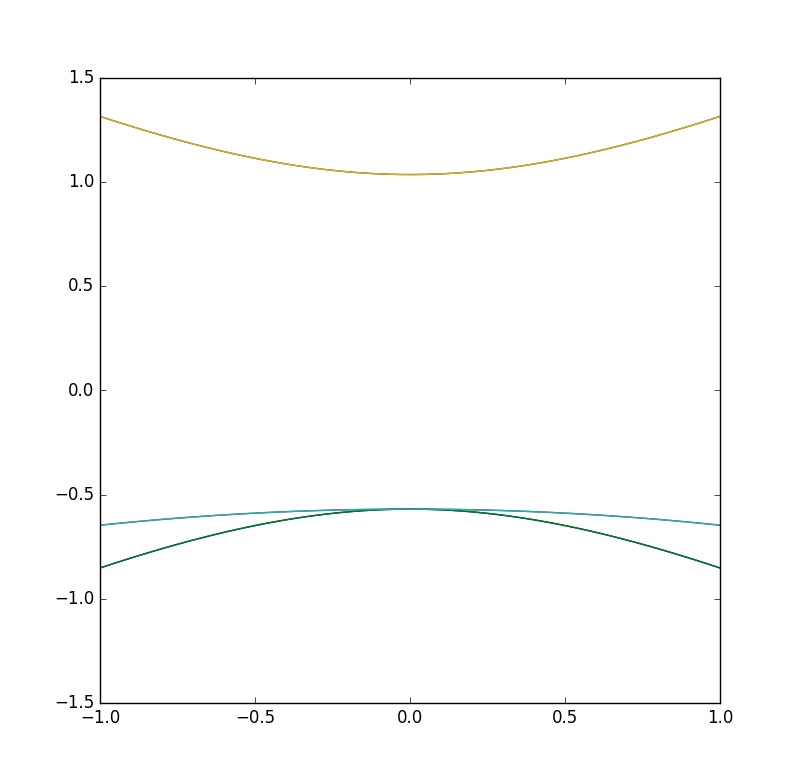
\includegraphics[width=0.6\linewidth]{cdte.png}
    \caption{На графике изображены ветви спектра CdTe в модели Кейна для параметров
             из \cite{Novik2005}. По оси абсцисс отложен волновой вектор в $\mathrm{nm}^{-1}$,
             по оси орбинат --- энергия в eV.}
\end{figure}

Таким образом, простая модель сильной связи воспроизводит известные свойства 
полупроводников со спин--орбитальным взаимодействием.

%\begin{equation}
%\scalebox{0.6}{%
%$
%H_v = \begin{pmatrix}
%       (t_\parallel + t_\perp)(\cos{p_x} + \cos{p_y}) + 2t\perp \cos{p_z} & 0 &
%       -\frac{1}{\sqrt{3}}(t_\parallel - t_\perp)(\cos{p_x} - \cos_{p_y}) & 0 \\
%
%       0 & \left(\frac{t_\parallel}{3} + \frac{5t_\perp}{3}\right)(\cos{p_x} + \cos{p_y}) + 
%                   \left(\frac{2t_\perp}{3} + \frac{4t_\parallel}{3}\right)\cos{p_z} & 
%       0 & -\frac{1}{\sqrt{3}}(t_\parallel - t_\perp)(\cos{p_x} - \cos_{p_y})\\
%       -\frac{1}{\sqrt{3}}(t_\parallel - t_\perp)(\cos{p_x} - \cos_{p_y}) & 0 &
%      \left(\frac{t_\parallel}{3} + \frac{5t_\perp}{3}\right)(\cos{p_x} + \cos{p_y}) + 
%                   \left(\frac{2t_\perp}{3} + \frac{4t_\parallel}{3}\right)\cos{p_z} & 0 \\
%       0 & -\frac{1}{\sqrt{3}}(t_\parallel - t_\perp)(\cos{p_x} - \cos_{p_y}) & 
%       0 & (t_\parallel + t_\perp)(\cos{p_x} + \cos{p_y}) + 2t\perp \cos{p_z}
%      \end{pmatrix}
%$
%}
%\end{equation}


%Гамильтониан имеет вид
%\begin{multline}
%   \label{well_model_ham}
%   H  = \sum_{m,n} (E_s + 4t_s) s_{mn}^{\dagger} s_{mn} - t_s s_{mn}^{\dagger}
%                          (s_{m+1,n} + s_{m-1,n} + s_{m,n+1} + s_{m,n-1}) \\
%          + t_{sp} s_{mn}^{\dagger} (-p_{m+1,n}^x + p_{m-1,n}^x - p^y_{m,n+1} + p^y_{m,n-1})
%                                                                + \mathrm{h.c.}  \\
%          + (p_{mn}^x)^{\dagger}(t_{\parallel}(p_{m+1,n}^x + p_{m-1,n}^x) +
%                                 t_{\perp} (p^x_{m,n+1} + p^x_{m,n-1})) \\
%          + (p_{mn}^x)^{\dagger}(t_{\perp}(p_{m+1,n}^y + p_{m-1,n}^y) +
%                                 t_{\parallel} (p^y_{m,n+1} + p^y_{m,n-1})) \\
%          + (p_{mn}^z)^{\dagger} t_3 (p_{m+1,n}^z + p_{m-1,n}^z +
%                                p^z_{m,n+1} + p^z_{m,n-1}) \\
%          -\frac{E_{SO}}{3}
%                \begin{matrix}
%                    \left(\begin{matrix}
%                        p_x^\dagger & p_y^\dagger & p_z^\dagger
%                    \end{matrix}\right) \\
%                    \\
%                    \\
%                \end{matrix}
%        		\left(\begin{matrix}
%        			1 & i & -1 \\
%        			-i & 1 & i \\
%        			-1 & -i & 1
%        		\end{matrix} \right)
%                \left(\begin{matrix}
%                    p_x \\ 
%                    p_y \\
%                    p_z
%                \end{matrix}\right) + \\
%        + \text{всё то же самое с переворотом проекции спина}
%\end{multline}
%
%Тогда спин--орбитальный гамильтониан запишется так:
%\begin{equation}
%	H_{\mathrm{full}} = -\Delta E_{SO} 
%			(a_{\frac{1}{2}, \frac{1}{2}}^\dagger a_{\frac{1}{2}, \frac{1}{2}} +
%			a_{\frac{1}{2}, -\frac{1}{2}}^\dagger a_{\frac{1}{2}, -\frac{1}{2}})
%\end{equation}
%После простого преобразования получается последнее слагаемое в \eqref{well_model_ham}.

    \section{Реконструкция края}
В данном разделе рассматривается реконструкция края (аналогично \cite{Wang2017}) 
в модели сильной связи из \cite{Bernevig2006}.

Реконструкцией края (edge reconstruction) называется следующее явление.

    \newpage
\section{Заключение}
Краевые состояния оказываются устойчивыми не просто к слабому потенциальному беспорядку, 
но и к беспорядку, создающему ненулевую плотность состояний в щели. 

    \newpage
    \appendix
    \newpage
\section{Уровни размерного квантования\\ в квантовой яме HgTe}
\label{app:dim_quant}
Гамильтониан Кейна имеет вид
\begin{equation}
    \label{kane_ham}
    H = \begin{pmatrix}
                E_c + \frac{\hbar^2 k^2}{2m_s}E_{2\times 2} & T \\
                T^\dagger & E_v + H_{L}
        \end{pmatrix}
\end{equation}
\begin{equation*}
    H_L = -\frac{\hbar^2}{2m_0}\left[
            \left(\gamma_1 + \frac{5}{2}\gamma_2\right)k^2 -
            2\gamma_2(\vec{k} \cdot \vec{J})^2 - \right. 
            - \left.2(\gamma_3 - \gamma_2)(\{J_x J_y\} + \{J_x J_z\} + \{J_y J_z\})
            \vphantom{\frac{1}{2}}\right]
\end{equation*}
\begin{equation*}
    T = P\begin{pmatrix}
           -\frac{1}{\sqrt{2}}k_{+} & \sqrt{\frac{2}{3}}k_z  
                    & \frac{1}{\sqrt{6}} k_{-} & 0 \\
            0 & -\frac{1}{\sqrt{6}} k_{+} 
                    & \sqrt{\frac{2}{3}}k_z & \frac{1}{\sqrt{2}} k_{-} 
         \end{pmatrix}
\end{equation*}
Так как
коэффициенты в гамильтониане Кейна зависят явным образом от $z$, нужно сделать замену
$k_z \to i\partial_z$. При этом, чтобы гамильтониан остался эрмитовым,
$\frac{k_z^2}{2m} \to -\partial_z \frac{1}{2m} \partial_z$ (и аналогично --- для других
членов). Все величины, зависящие от $z$, равны значениям для HgTe при $-d/2 < z < d/2$,
для CdTe --- в противном случае.

Уровни размерного квантования можно относительно просто найти для $k_x, k_y = 0$. В этом 
случае гамильтониан значитально упрощается. Уровни тяжёлых дырок оказываются полностью
отщеплёнными для каждой проекции спина и описываются эффективным гамильтонианом
\begin{equation}
    H_{\mathrm{HH}} = E_v(z) + \frac{1}{2m}
                        \frac{\partial}{\partial z} 
                        (\gamma_1(z) - 2\gamma_2(z)) 
                        \frac{\partial}{\partial z} 
\end{equation}
Также отщепляются $s$--зона вместе с зоной лёгких дырок. Они описываются эффективным
гамильтонианом 
\begin{equation}
    H_{\mathrm{s,LH}} = \begin{pmatrix}
                            E_c - \frac{\hbar^2}{2m}
                                 \frac{\partial}{\partial z}(1 + 2F) 
                                 \frac{\partial}{\partial z} &
                                 \sqrt{\frac{2}{3}}P k_z \\
                                 \sqrt{\frac{2}{3}}P k_z &
                                 E_v +  \frac{\hbar^2}{2m}
                                 \frac{\partial}{\partial z}(\gamma_1 + 2\gamma_2)
                                 \frac{\partial}{\partial z} 
                        \end{pmatrix}
\end{equation}
Для обоих гамильтонианов можно получить алгебраические уравнения на уровни энергии. Эти
уравнения решаются численно.

    \section{Отсутствие рассеяния для крамерсовского дублета}
\label{app:kramers_doublet}
Нетрудно проверить, что для частицы со спином $\frac{1}{2}$
\begin{equation}
    \bra \chi | T\psi \ket = -\bra \psi | T\chi\ket
\end{equation}
Тогда $\bra \psi | \hat{A}  | T\psi \ket = 0$ для любого 
$|\psi \ket$, если
$\hat{A}$ удовлетворяет условию $-T\hat{A}^\dagger T = \hat{A}$.
Действительно,
\begin{equation}
    \bra \psi | \hat{A}  | T\psi \ket = \bra \hat{A}^\dagger \psi | T\psi \ket = 
       -\bra \psi | T \hat{A}^\dagger| \psi \ket = -\bra \psi | (-T\hat{A}^\dagger T) | T\psi \ket
\end{equation}
Оператор эволюции $T$--инвариантной системы удовлетворяет именно такому условию:
\begin{equation}
    -T\hat{U}T = U^{-1} = U^\dagger
\end{equation}
Поэтому рассеяние $|\psi\ket$ и $|T\psi\ket$ друг в друга запрещено.

    \section{Вычисления для точечной примеси}
\subsection{Энергия связанного состояния}
\label{app:impurity}
Уравнения \eqref{imp_equation} принимают вид
\begin{align}
        &G(\omega,0,0)_{11} = \int \frac{d^2 p}{(2\pi)^2} 
            \frac{\omega + \xi + \frac{1}{m}(2 - \cos{p_x} - \cos{p_y})}
                 {\omega^2 - E_p^2} =\frac{1}{\Delta E}, \label{local_state_eq:1}\\
        &G(\omega,0,0)_{22} = \int \frac{d^2 p}{(2\pi)^2} 
            \frac{-\omega + \xi + \frac{1}{m}(2 - \cos{p_x} - \cos{p_y})}
                 {\omega^2 - E_p^2} =-\frac{1}{\Delta E}, \label{local_state_eq:2}
\end{align}
Интегралы можно взять приближённо в круге радиуса $p_{\mathrm{max}}$,
если учесть, что при малых $p$ спектр близок к 
коническому. Можно считать, что $p_{\mathrm{max}} \sim 1$. После интегрирования получается
выражение \eqref{approx_green_func}. Используя его, мы получили \eqref{impurity_energy}.


Покажем, что для большого $\Delta E$ и $\xi > 0$ связанного состояния в щели нет. 
В этом случае $\delta \omega < 0$ и логарифм в формуле \eqref{approx_green_func} ---
большое положитальное число. При этом в правой части \eqref{local_state_eq:1} стоит
$\frac{1}{\Delta E} \to 0$. Это значит, что равенство не может быть выполнено.


\subsection{Волновая функция связанного состояния}
Волновые функции даются компонентами свободной функции Грина \eqref{green_function}.
Их можно вычислить с помощью формального трюка. Определим новую функцию
$F(x,y)$:
\begin{equation}
    F(x,y) = \equiv \int \frac{d^2 p}{(2\pi)^2} 
            \frac{e^{ip_x x + ip_y y}}{\omega^2 - E_p^2} 
\end{equation}
Несложно понять, что компоненты функций Грина выражаются (точными соотношениями)
 через $F(x,y)$. А именно,
\begin{equation}
    \label{differences}
    \begin{split}
        G_{11} & = (\omega + \xi) F(x,y) - 
            \frac{1}{m}(F(x+1,y) + F(x-1,y) + F(x,y+1) + F(x, y-1) - 4F(x,y))\\
        G_{21} & = -it(F(x+1,y) - F(x-1,y)) + t(F(x,y+1) - F(x,y-1))
    \end{split}
\end{equation}
С другой стороны, $F(x,y)$ может быть вычислена приближённо. Если разложить 
выражение в знаменателе около $p = 0$ и распространить интегрирование до $\infty$, то получится
сходящийся и берущийся интеграл.
\begin{equation}
    F(x,y) \approx -\int \frac{p\,dp\,d\cos{\theta}}{(2\pi)^2} 
        \frac{e^{ipr\cos{\theta}}}{\xi^2 - \omega^2 - (4t^2 + \frac{\xi}{m})p^2} = 
        -\frac{1}{2\pi} \frac{1}{4t^2 + \frac{\xi}{m}}
        K_0 \left(\sqrt{\frac{\xi^2 - \omega^2}{4t^2 + \frac{\xi}{m}}}R \right)
\end{equation}
Разности \eqref{differences} можно аппроксимировать производными. Пользуясь тем, что
$K_0(x)$ --- решение модифицированного уравнения Бесселя, получим 
\begin{equation}
    \begin{split}
        G_{11} & = -\frac{1}{2\pi} \frac{1}{4t^2 + \frac{\xi}{m}}
        \left( \omega + \xi - \frac{1}{m} \frac{\xi^2 - \omega^2}{4t^2 + \frac{\xi}{m}} \right)
        K_0 \left(\sqrt{\frac{\xi^2 - \omega^2}{4t^2 + \frac{\xi}{m}}}R \right)\\
        G_{21} & = \frac{it}{\pi} \sqrt{\frac{\xi^2 - \omega^2}
                                     {(4t^2 + \frac{\xi}{m})^{3}}}
        K_0' \left(\sqrt{\frac{\xi^2 - \omega^2}{4t^2 + \frac{\xi}{m}}}R \right)e^{i\theta}
    \end{split}
\end{equation}

    \section{Коэффициенты Клебша--Гордана}
\label{app:tb}
Состояния с определённым полным моментом выражаются через $p_x$, $p_y$, $p_z$ орбитали через
коэффициенты Клебша--Гордана:
\begin{equation}
	\label{transform1}
	\begin{gathered}
        \Psi_{\frac{3}{2},\frac{3}{2}} = \frac{X + iY}{\sqrt{2}}\alpha\\
        \Psi_{\frac{3}{2}, \frac{1}{2}} = \sqrt{\frac{1}{3}}\frac{X + iY}{\sqrt{2}}\beta -
                                         \sqrt{\frac{2}{3}} Z\alpha\\
        \Psi_{\frac{3}{2}, -\frac{1}{2}} = -\sqrt{\frac{1}{3}}\frac{X - iY}{\sqrt{2}}\alpha -
                                         \sqrt{\frac{2}{3}} Z\beta\\
        \Psi_{\frac{3}{2},-\frac{3}{2}} = -\frac{X - iY}{\sqrt{2}}\beta
	\end{gathered}
\end{equation}
\begin{equation}
	\label{transform2}
	\begin{gathered}
        \Psi_{\frac{1}{2}, \frac{1}{2}} = \sqrt{\frac{2}{3}}\frac{X + iY}{\sqrt{2}}\beta +
                                         \sqrt{\frac{1}{3}} Z\alpha\\
        \Psi_{\frac{1}{2}, -\frac{1}{2}} = -\sqrt{\frac{2}{3}}\frac{X - iY}{\sqrt{2}}\alpha-
                                         \sqrt{\frac{1}{3}} Z\beta\\
	\end{gathered}
\end{equation}

Здесь $X,Y,Z$ --- атомные орбитали, $\alpha,\beta$ --- состояния со спином вверх и вниз.

\afterpage{%
    \clearpage% Flush earlier floats (otherwise order might not be correct)
%    \thispagestyle{empty}% empty page style (?)
    \begin{landscape}% Landscape page
        \centering % Center table
        \vspace*{\fill}
        \begin{equation}
            \label{H_conduction}
            H_c = (E_s + \frac{1}{m_s}(3 - \cos{p_x} - \cos{p_y} - \cos{p_z}))I_{2\times2}
        \end{equation}
        \begin{equation}
            \label{T_matrix}
            T = P\begin{pmatrix}
                    -\frac{1}{\sqrt{2}}(\sin{p_x} + i\sin{p_y}) & \sqrt{\frac{2}{3}}\sin{p_z} &
                     \frac{1}{\sqrt{6}}(\sin{p_x} - i\sin{p_y}) & 0 \\  
                    0 & -\frac{1}{\sqrt{6}}(\sin{p_x} + i\sin{p_y}) & 
                    \sqrt{\frac{2}{3}}\sin{p_z} & \frac{1}{\sqrt{2}}(\sin{p_x} - i\sin{p_y}),
                 \end{pmatrix},
        \end{equation}
        \begin{equation}
            \label{H_valence}
            H_v = 
            \begin{pmatrix}
                (t_\parallel + t_\perp)(\cos{p_x} + \cos{p_y}) + 2t_\perp \cos{p_z} & 0 &
                -\frac{1}{\sqrt{3}}(t_\parallel - t_\perp)(\cos{p_x} - \cos_{p_y}) & 0 \\
                0 & \left(\frac{t_\parallel}{3} + \frac{5t_\perp}{3}\right)(\cos{p_x}+\cos{p_y})+ 
                              \left(\frac{2t_\perp}{3} + \frac{4t_\parallel}{3}\right)\cos{p_z} &
                0 & -\frac{1}{\sqrt{3}}(t_\parallel - t_\perp)(\cos{p_x} - \cos_{p_y})\\
                -\frac{1}{\sqrt{3}}(t_\parallel - t_\perp)(\cos{p_x} - \cos_{p_y}) & 0 &
               \left(\frac{t_\parallel}{3} + \frac{5t_\perp}{3}\right)(\cos{p_x} + \cos{p_y}) + 
                       \left(\frac{2t_\perp}{3} + \frac{4t_\parallel}{3}\right)\cos{p_z} & 0 \\
                0 & -\frac{1}{\sqrt{3}}(t_\parallel - t_\perp)(\cos{p_x} - \cos_{p_y}) &
                0 & (t_\parallel + t_\perp)(\cos{p_x} + \cos{p_y}) + 2t_\perp \cos{p_z}
            \end{pmatrix}
        \end{equation}
    \vspace*{\fill}
    \end{landscape}
    \clearpage% Flush page
}

    \newpage
    \bibliography{/home/ksenia/notes/science/top_ins/literature}
\end{document}
